%\motto{Use the template \emph{chapter.tex} to style the various elements of your chapter content.}
\chapter{Physikalische Grundlagen}
\label{physics} % Always give a unique label

\chapterauthor{Amanda Hagan, Lucie Hartmann, Leon Lukacin, Ole Pross}

\abstract{some abstract}

\section{(Einführung in die Quantenmechanik für das Quantencomputing)}
\subsection{Motivation und Abgrenzung zur klassischen Physik }
\subsection{Wichtige Konzepte der Quantenmechanik }
\subsubsection{\textit{\textit{Zustände und Wellenfunktion} }}
\subsubsection{\textit{Observable und Messung}} 
\subsubsection{\textit{(Zeitentwicklung und Schrödingergleichung??)} }

\section{Zentrale Quantenphänomene }
\subsection{Superposition }

\begin{itemize}
\item Licht verhält sich wie Welle (Doppelspaltexperiment) und Teilchen (Photon)
\item Welle Teilchen Dualismus
\item Beispiel mit Schrödingers Katze
\item In beiden Zuständen bis gemessen wird
\item Teilchen z.B. an zwei Orten gleichzeitig, aber auch andere (sich ausschließende) Eigenschaften parallel -> Superposition -> Teilchen in allen möglichen Zuständen gleichzeitig
\item Einwirkung von außen oder Messung zerstört Superposition
\item Heisenbergsche Unschärferelation
\item Beide Zustände der Superposition haben jeweils einen Anteil, der genaue Wert eines Anteils ist nicht bekannt
\item Mit einer Wahrscheinlichkeit abhängig vom Anteil nimmt ein Teilchen einen der beiden Zustände an

\item Schrödingergleichung/Wellenfunktion
\item Linearkombination (widersprüchlicher) Zustände z.B. 0 und 1/ tot und lebendig
Bei Messung erfolgt Kollaps der Wellenfunktion -> am Ende ein Zustand
\item Wellenfunktion beschreibt ein quantenmechanisches System und enthält alle Informationen über dieses System
\item Eigenvalues und Eigenstates
\end{itemize}

\subsection{Quanteninterferenz}

\begin{itemize}
\item Interferenzmuster aus Doppelspaltexperiment -> Wahrscheinlichkeitsamplitude
Wahrscheinlichkeitsamplituden können sich verstärken oder auslöschen (konstruktiv/destruktiv)
\item Interferometer
\item Einzelnes Photon löst allein Interferenz aus -> entgegen Intuition -> Photon muss in Superposition sein
\item Messung zerstört Verhalten als Welle -> nur noch als Teilchen
Nutzbar in Gattern
\item Tunneleffekt
\end{itemize}

\subsection{Verschränkung }

Das Konzept der Verschränkung (engl. ``entanglement'') beschreibt gewissermaßen die Korrelation mehrerer Qubits miteinander, das heißt sie hängen in einem besonderen Maße zusammen. \\
Für einen erleichterten Einstieg soll ein Beispiel anhand zweier gewöhnlicher Münzen gemacht werden. Werden zwei gewöhnliche Münzen geworfen, hat man vier mögliche Ausgänge für den Münzwurf, bei denen H für Kopf und T für Zahl stehen sollen: HH, HT, TH, TT. \\
Alle Varianten der Ausgänge haben hierbei eine identische Wahrscheinlichkeit von 25\%. Sind diese zwei Münzen jedoch in einem verschränkten Zustand  $\frac{1}{\sqrt{2}} \left( \lvert HH \rangle + \lvert TT \rangle \right)$, sind hierbei nur zwei Ausgänge möglich, die beide jeweils eine 50\%-Wahrscheinlichkeit haben, nämlich HH oder TT. \\
Diese Verschränkung ist unabhängig von der räumlichen Nähe der Münzen und kann über große Distanzen hinweg wirken. Weiß man das Ergebnis der einen Münze, so weiß man automatisch auch immer das Ergebnis der anderen Münze. Im Bereich der Quantenmechanik ist genau dies bezogen auf diverse Teilchen anstelle der Münzen möglich. 
Das Phänomen der Verschränkung ist jedoch ein reines Quantenphänomen, das keine Erklärung in der klassischen Physik besitzt. \\
Eine Vermutung über die Natur der Verschränkung besteht aus der sofortigen Informationsübertragung zweier Teilchen, die über die Schnelligkeit der Lichtgeschwindigkeit hinausgeht, was jedoch als widerlegt gilt. Stattdessen teilen Teilchen nicht-klassische Information während der Verschränkung, die im Messprozess beobachtet werden kann. \\
Eine weitere frühe Interpretation, bekannt unter dem Namen ``Hidden Variable Theory'', nahm an, dass Teilchen beim Erzeugen mit verbogenen Eigenschaften erschaffen werden, die Messergebnisse deterministisch bestimmen. Beispielsweise wäre hierfür der Zerfall eines Teilchens in zwei Teilchen. Auf Basis der Impulserhaltung kann man durch die Messung des Impuls des einen Teilchens auf den Impuls des anderen Teilchens schließen, da der Gesamtimpuls vorher bekannt ist. 
\cite{hughes_quantum_2021}
% Quantum Computing for the Quantum Curious - Hughes et al. - 2021
\\

Das Problem dieser Theorie findet sich jedoch in Bell's Theorem, das zeigt, dass wenn die Welt durch diese versteckten Variablen beschrieben wäre, gewisse mathematische Ungleichungen in Experimenten eingehalten werden müssten. 
Diese gelten als Einschränkungen für alle lokal-realistischen Theorien, d.h. Theorien, die annehmen, dass Lokalität und Realismus gelten. \\
Lokalität bedeutet hierbei, dass es keinen Einfluss gibt, der sich schneller als mit Lichtgeschwindigkeit ausbreiten kann. \\
Realismus bezieht sich auf die Annahme, dass physikalische Größen zu jedem Zeitpunkt definierte Werte besitzen, unabhängig davon, ob diese gemessen werden. 
Die quantenmechanische Verschränkung erfüllt diese Annahmen durch die ``spukhafte Fernwirkung'' jedoch nicht, da es eine scheinbar unmittelbare Verbindung über sehr große Distanz hinweg gibt. Dem Lokalitätsprinzip entsprechend, könnten zwei Systeme sich nur dann beeinflussen, wenn sie einen Kontakt oder ein physikalisches Feld haben, das sie verbindet. Quantenobjekte haben jedoch durch die mangelnde Lokalität keine klassische Kausalität, sondern nur die Beobachtung, dass die Ergebnisse immer korrelieren, auch wenn sie räumlich weit voneinander getrennt sind.

Da die Grenzen der Bell-Ungleichung also nicht auf gemessene Experimente zutreffen, kann keine lokal-realistische Theorie das quantenmechanische Phänomen der Verschränkung erklären. Die Resultate stimmen mit der Quantenmechanik überein, anstatt mit lokalen Theorien wie der Hidden Variable Theory. 

Basierend hierauf ergibt sich das Dilemma, dass Realismus und Lokalität nicht beide gleichzeitig gelten können. Diese Schlussfolgerung führt jedoch zu tiefergehenden philosophischen Fragen über die Realität, die an dieser Stelle nicht weiter behandelt werden sollen.
Unabhängig davon findet die Verschränkungen Anwendungen in moderner Quantentechnologie, wie in der Quantenkryptographie oder Quanten-Teleportation.  
\cite{homeister_quantum_2022}
% Quantum Computing verstehen: Grundlagen - Anwendungen - Perspektiven - Homeister - 2022
\\

Um ein Beispiel für die Quantenverschränkung in der Praxis zu machen, soll an dieser Stelle noch  die spontane parametrische Fluoreszenz (engl. ``spontaneous parametric down-conversion, SPDC'') genannt werden. Bei diesem Prozess trifft ein Photon aus einem Laser auf ein nichtlineares Kristallmaterial. Dadurch spaltet sich das Photon in zwei neue Photonen, wobei die Polarisation der neuen Photonen miteinander verschränkt sind, sodass man typischerweise folgenden Zustand erhält:
$\frac{1}{\sqrt{2}} \left( \lvert H \rangle_A \lvert H \rangle_B + \lvert V \rangle_A \lvert V \rangle_B \right)$
Misst man also die Polarisation des Photons A, kennt man ebenfalls die Polarisation des Photons B, jedoch ohne dass dies klassisch bereits festgelegt war.
\cite{hughes_quantum_2021}
% Quantum Computing for the Quantum Curious - Hughes et al. - 2021



\section{Quantenmessung }
\subsection{Grundlagen der Quantenmessung (projektive Messungen, Messoperatoren)}

Die Messung in der Quantenmechanik unterscheidet sich grundlegend von der Messung in der klassischen Physik, einerseits durch die Auffassung der Grundkonzepte der Quantenmechanik, andererseits durch die mathematische Beschreibung und Interpretation der Messergebnisse.
In der klassischen Welt wird das Verhalten eines Systems nicht durch das alleinige Beobachten des Systems beeinflusst; ein Ball beispielsweise wird sein Verhalten und seine Flugkurve nach einem Schuss nicht verändern, unabhängig davon, ob jemand dabei zusieht oder nicht.
In der Quantenwelt hingegen sind die gemessenen Objekte (z.B. Photonen) winzig klein und die entsprechenden Messgeräte verhältnismäßig groß, sodass schon alleine deshalb die Messung zwangsläufig den Zustand eines Quantensystems beeinflussen wird. 
Dass eine Messung den Zustand des Quantensystems verändert und das Ergebnis dieser Messung zufällig ist, ist im Rahmen des zweiten Postulats der Quantenmechanik eine zentrale Annahme, die in diesem Kapitel weiter erörtert werden soll. Als Observablen- oder Messwertpostulat ist es das zentrale Postulat für die Messung im gegebenen Rahmen.

Das zweite Postulat besagt, dass eine Quantenmessung einer Projektion des Zustandes $\ket{\psi}$ auf eine Basis $\ket{|v_i|}$ entspricht. Mit der Wahrscheinlichkeit $|\braket{v_i|\psi}|^2$ erhalten wir das Ergebnis $v_i$. Das System befindet sich dann im Zustand $\ket{v_i}$. \cite{lvovsky_quantum_2018} 
% Lvovsky - Quantum Physics - 2018 - Kapitel 1.4.1 The Measurement Postulate
\newline Dieses Konzept wird auch 'projektive Messung' genannt, da die Messung des Zustandes auf einen Basiszustand projiziert wird, wobei die Begriffe der Projektion und der Basiszustände noch weiter erläutert werden sollen. \\
\\

Ein Quantensystem wird innerhalb einer bestimmten Basis gemessen.Der Begriff 'Basiszustand' bezieht sich hierbei auf die möglichen Zustände eines Systems, die insgesamt die Basis bilden (beispielsweise $\ket{v_1}$ oder $\ket{v_2}$) und bei der Messungen angenommen werden können.
Beim Messen springt das System in einen der Basiszustände. 
Wird hierbei der Wert $v_i$ gemessen, so springt das System in den Zustand $\ket{v_i}$. Das Messergebnis ist also der Zustand $\ket{v_i}$. 
Dabei wird die Information, welche Zustände gemessen werden und welche entsprechenden Zahlenwerte ihnen zugeordnet werden, in einem 'Observable Operator' zusammengefasst. 
Dieser Observable Operator, der die Basis der Messungen beschreibt und die möglichen Werte der Messung enthält, kann folgendermaßen dargestellt werden: \\
\\
\begin{equation}
\hat{V} = \sum_i v_i \, \ket{v_i}\bra{v_i}
\end{equation}.
\\ 
\\
Jeder Zustand $\ket{v_i}$ ist hierbei ein Eigenzustand dieses Operators. Der dazugehörige Eigenwert $v_i$ ist der Zahlenwert der Messung, den man bei der Messung des Zustandes erhält. 
Die Zuordnung eines Wertes ist für einige Messgrößen (bspw. der Ort eines Teilchens im Raum) natürlich, für andere (z.B. die Polarisation eines Photons) weniger. Trotzdem wird auch in weniger natürlichen Fällen  eine Zahl zugeordnet, so beispielsweise
+1 für eine horizontale $\ket{H}$ und -1 für eine vertikale $\ket{V}$ Polarisation. Eine Observable kann für jede messbare Größe (Ort, Energie, Puls, Spin, etc.) definiert werden. Eine Ausnahme bildet hierbei die Zeit, da diese in der Quantenmechanik nicht als Observable definiert und behandelt wird.
Daher gibt es keinen Zeit-Operator oder Eigenzustände der Zeit. Die Zeit dient lediglich als kontinuierliche Variable zur Beschreibung der Entwicklung des Quantensystems. 
\cite{lvosvsky_quantum_2018} 
% Lvovsky - Quantum Physics - 2018 - Kapitel 1.9.1 Observable Operators
\\
\\

Projektive Messungen werden also durch eine Observable M beschrieben. Seien die Eigenwerte m die möglichen Ergebnisse der Messung und $P_m$ die zugehörigen Projektoren, kann M geschrieben werden als:
\begin{equation}
    M = \sum_m mP_m
\end{equation}
Hierbei sind $P_m$ die orthogonalen Projektoren auf den Eigenraum von M. Jeder Projektor projiziert auf einen Unterraum des Hilbertraums, der zu einem bestimmten Eigenwert m gehört. Diese Formel bildet die verallgemeinerte Darstellung der zuvor genannten Formel zur Darstellung der Observablen. % Check & umschreiben
Es gelten daraus folgende Grundregeln: \\ \\
\begin{enumerate}
\item Die Gesamtwahrscheinlichkeit aller Messungen (Projektoren) ergeben in Summe 1, d.h. sie decken den gesamten Zustandsraum ab. Jeder mögliche Zustand wird durch eine Kombination der Projektoren beschrieben und bildet in Summe den Einheitsoperator. \\
\item Die Wahrscheinlichkeit einer Messung m ergibt sich aus folgender Formel:
\begin{equation}
    p(m) = \langle \psi \mid P_m \mid \psi \rangle
\end{equation}
Hierbei ist p(m) die Wahrscheinlichkeit, dass die Messung des Systems im Zustand $\ket\psi$ das Ergebnis m ergibt. Das ist mathematisch das s.g. Bornsche Wahrscheinlichkeitsgesetz.
Es ist das Quadrat der Länge der Projektion von $\ket\psi$ auf den m-Unterraum. Es berechnet also die Länge der Projektion von $\ket\psi$ auf den Eigenraum von m. \\
\item Nach einer Messung mit Ergebnis m kollabiert der Zustand $\ket\psi$ in einen Zustand, der der Messung entspricht. Dies wird auch Projektionspostulat genannt. Die Projektion dieses Zustandes muss wieder normalisiert werden, um wieder einen Zustand mit der Norm 1 zu erhalten.
Da wiederholte Messungen jedoch im Bereich des Quantumcomputing geringe Relevanz hat, wird auf die wiederholte Messung nicht weiter eingegangen. \\ 
\end{enumerate}

In kurz greift man bei der Messung eines Zustandes $\ket\psi$ also nur den Teil aus dem gesamten Zustandsvektor heraus, den man misst. Es wird der Anteil extrahiert, der zugehörig zum gemessenen Eigenwert ist, also die Projektion $P_m \ket\psi$. Der Zustand wird bei der Messung also in seine Bestandteile entsprechend der verschiedenen Eigenräume zerlegt. Um hieraus wieder einen gültigen und normierten Zustand zu erhalten, muss dieser Vektor mit seiner eigenen Länge normiert werden. Da dies jedoch nur zur weiteren Arbeit mit demselben Quantensystem relevant ist, wird die Normierung nicht weiter berücksichtigt und es wird stattdessen auf wiederholte Messungen verwiesen.
\cite{kasirajan_fundamentals_2021} 
%Fundamentals of Quantum Computing: Theory and Practice – Kasirajan (Kapitel zu Projective Measurements)

Um ein Beispiel für den Messprozess und den Zerfall auf den Eigenzustand bei der projektiven Messung zu machen, soll ein Photon auf einen Polarizing Beam Splitter (PBS) treffen. Dieser lässt horizontal polarisiertes Licht passieren, aber reflektiert vertikal polarisiertes Licht.
Betrachtet man einen Lichtstrahl aus der klassischen Physik, würde man erwarten, dass dieser sich teilt - ein Teil des Lichtes würde reflektiert werden, ein anderer Teil würde passieren. Ein Photon als kleinster Teil des Lichts kann jedoch nicht weiter geteilt werden.
Dementsprechend ist das Ergebnis zufällig: das Photon wird mit einer gewissen Wahrscheinlichkeit passieren oder reflektiert werden. Das Photon entscheidet sich bei der Messung, ob es horizontal oder vertikal polarisiert sein wird und springt bei der Messung in den gewählten Zustand.
Man könnte auch sagen durch die Messung wird der Superpositionszustand auf einen der möglichen Eigenzustände reduziert. Die Superposition selbst liegt nicht im Eigenraum, sondern ist eine Überlagerung der Zustände aus den Eigenräumen, wobei ``horizontal'' und ``vertikal'' im Eigenraum mit ihrem jeweiligen Eigenwert liegen. Hierbei zerfällt der Ursprungszustand, sodass dies bei folgenden PBS nicht erneut vonstatten gehen könnte - das Photon wird den hierbei gewählten Zustand beibehalten.
Es gibt ab diesem Punkt keine weiteren zufälligen Zustandsänderungen. 
\cite{lvovsky_quantum_2018}
% Quantum Physics – Lvovsky – 2018 (Kapitel 1.4.1 The Measurement Postulate)

\subsection{Nichtdeterminismus}

Das oben beschrieben Phänomen der zufälligen Messung ist auf den Nichtdeterminismus der Quantenmessung zurückzuführen. Das bedeutet, dass das Ergebnis der Messung zufällig ist. Man erhält den Wert $\ket v_i$ mit einer gewissen Wahrscheinlichkeit.
Je besser der Zustand $\ket \psi$ zu einem Messzustand $\ket v_i$ passt, desto wahrscheinlicher ist das Ergebnis $v_i$. Mit Hilfe des Observable Operators können Werte der klassischen Statistik berechnet werden, so der Erwartungswert, die Varianz bzw. die Unschärfe der Messung (Standardabweichung). 
Klassisch statistische Kennzahlen lassen sich mit klassischen Operationen berechnen. Entsprechend ist die statistische Verteilung der Messergebnisse leicht zu berechnen. 
\\ \\
Um hierbei auf das Beispiel der Photonen zurückzukommen, führen wir ein, dass die horizontale Polarisierung des Photons dem Wert +1 zugeordnet wird, die vertikale Polarisierung dem Wert -1.
Ein diagonal polarisiertes Photon (45°) hat entsprechend eine 50\% Chance den PBS zu passieren (+1) oder reflektiert zu werden (-1). Bei der wiederholten Messung dieses Prozesses, ist der Mittelwert 0, da sich beide Superpositionen ausgleichen.
Die Varianz entspricht einem Wert von 1, da die Messung immer um +1 oder -1 vom Mittelwert (0) abweicht.
In der klassischen Physik sind solche Messungen deterministisch vorhersehbar. Für einzelne Photonen gibt es den Zufall, für eine Vielzahl von Photonen als Licht gibt es jedoch feste Erwartungen und Regeln.
Entsprechend ist es auch im Quantensystem. Mit einer Vielzahl an Photonen wird die relative Unsicherheit sehr klein und das Verhalten erscheint klassisch und stabil, obwohl die Photonen im Kleinen in Form der Einzelphotonen vom Zufall beherrscht sind.
Die Quantenfluktuationen verschwindend relativ gesehen also im großen Maßstab durch die wiederholte Messung und eine klare Wahrscheinlichkeitsverteilung.
\cite{kasirajan_fundamentals_2021}
% Quantum Physics – Lyvovsky – 2018 (Kapitel 1.9.2 Observable Operators)
\\ \\
Erwähnenswert im Rahmen der Messung ist weiterhin das 'Heisenberg Uncertainty Principle'. In der klassischen Physik ist eine Unsicherheit im Rahmen der Messung Folge eines ungenauen Messapparates, die durch eine Verbesserung des Apparates selbst verringert werden kann.
Dies gilt jedoch im Kontext der Quantenmechanik nicht. Hierbei kann ein Apparat präzise auf die Messung eines Observablen abgestimmt sein, jedoch bei der Messung einer anderen Observablen durchweg schlecht abschneiden. \\
Möchte man zwei Größen gleichzeitig messen, beispielsweise Ort und Energie oder auch verschiedene Spins, so kann das möglich sein. Hierzu müssen jedoch zwei Observablen kommutieren, d.h. mathematisch verträglich sein, um gleichzeitig messbar sein zu können. \\
Ist dies der Fall, gibt es eine bestimmte Basis von Zuständen (Eigenbasis), in der beide Observablen gleichzeitig genau bestimmt werden können. Das System in diesem Zustand verändert seinen Zustand nicht, wenn beide Größen nacheinander gemessen werden, d.h. die Observablen sind kompatibel. \\
Wenn die Observablen jedoch nicht kommutieren, so gibt es keinen Zustand, bei dem man beide Größen gleichzeitig exakt wissen kann. Misst man hierbei A, wird das Ergebnis von B zufällig sein, da die Messung von B durch die Information über A gestört ist.
Das heißt bestimmte Paare von Größen können nicht gleichzeitig beliebig genau gemessen werden. 
Zwei Größen, die nicht kommutieren, sind z.B. Ort und Impuls eines Teilchens. Je genauer man den Ort kennt, desto ungenauer lässt sich der Impuls messen und umgekehrt. 
\cite{kasirajan_fundamentals_2021}
% Quantum Physics – Lyvovsky – 2018 (Kapitel 1.9.3 Uncertainty Principle)

\subsection{Messprozess}

Ein Prozess, der im Rahmen der Messung bereits mehrfach erwähnt, jedoch bisweilen noch nicht konkret benannt wurde, ist der Kollaps der Wellenfunktion. Dieser Prozess ist zentral für die Messung. 
Unter dem Kollaps der Wellenfunktion versteht man den Vorgang, bei dem der Zustand eines Quantensystems auf einen Basiszustand 'springt', das heißt der Zustand des Systems kollabiert auf einen der möglichen Messzustände. Die Wahrscheinlichkeit für den Wert, den man beim Kollaps erhält, ist durch die bereits genannte Bornsche Regel beschrieben.
Dies zeigt die Annahme der Quantenmechanik des Nichtdeterminismus, dass der Zufall grundlegend ist. Selbst mit perfekten Geräten kann der Zustand entsprechend nicht exakt vorhergesagt werden. 
\cite{lvovsky_quantum_2018}
% Quantum Physics – Lyvovsky – 2018 (Kapitel 1.4.1 The Measurement Postulate)
\\

Ein Quantenzustand ist also nur in abgeschottetem Zustand stabil. Um aus Perspektive der Außenwelt etwas über den Zustand des Systems zu erfahren, ist jedoch eine Messung nötig, wobei der genaue Zustand nicht ermittelt werden kann.
Die Superposition selbst wird durch die Messung zerstört und ein klassischer Zustand wird angenommen und beobachtet. Diese Messung ist außerdem für verschiedene Basen möglich und es kann entsprechend nur der Zustand bzgl. einer Basis gemessen werden, sofern die folgende Messung durch den Zerfall des Systems nicht weiter möglich ist.
Da die Messung nicht rückgängig gemacht werden kann, kann durch den Kollaps der Wellenfunktion dieselbe Messung nicht wiederholt werden.
\cite{homeister_quantum_2022}
% Quantum Computing verstehen: Grundlagen – Anwendungen – Perspektiven – Homeister – 2022 (Kapitel 2.8 Das Messen von Quantenregistern)
\\

Aus diesem Phänomen ergibt sich auch das No-Cloning-Theorem. Da das System selbst bei der Messung zerstört wird, kann das Qubit nicht erneut gemessen werden. Die Superposition selbst ist für dasselbe Qubit nicht mehr vorhanden. Die Messung kann entsprechend nur für ein identisches Qubit wiederholt werden.
Folglich dieser Logik kann ein Qubit in einem unbekannten Zustand nicht kopiert werden. Dies hat wichtige Konsequenzen für die praktische Anwendung, da simple Kopien, wie sie auf klassischen Computern möglich sind, durch die zuvor notwendige Messung der bestehenden Zustände nicht ohne Weiteres auf quantenbasierten Systemen ermöglicht werden.
\cite{hughes_quantum_2021}
% Quantum Computing for the Quantum Curious – Hughes et al. – 2021 – s. 36

\section{Mathematische Beschreibung von Qubits}

\subsection{Hilbertraum und Zustandsvektoren}
\textbf{Zustand eines Qubits} durch einen normierten Vektor in einem zwei-dimensionalen komplexen Hilbertraum.
\begin{itemize}
    \item Beschreibung des Hilbertraums:
    \begin{itemize}
        \item Komplexer Vektorraum mit Skalarprodukt.
    \end{itemize}
    \item Zustände als Basisvektoren.
    \item Allgemeine Qubit-Zustände als Linearkombination.
    \item Bedeutung der Normierung (Wahrscheinlichkeitsinterpretation und komplexe Koeffizienten).
\end{itemize}

\section*{Beschreibung des Hilbertraums}

Die mathematische Grundlage zur Beschreibung von Qubits bildet der sogenannte \textit{Hilbertraum}. In der Quanteninformationstheorie beschreibt dieser einen abstrakten, komplexen Vektorraum, der mit einem Skalarprodukt ausgestattet ist. Er dient als Trägerraum für alle möglichen Zustände eines quantenmechanischen Systems. In diesem Kapitel wird sich auf den einfachsten Fall beschränkt: den zweidimensionalen Hilbertraum $\mathcal{H}_2$, der zur Darstellung eines einzelnen Qubits verwendet wird.

Ein Hilbertraum ist per Definition ein vollständiger Vektorraum über dem Körper der komplexen Zahlen $\mathbb{C}$ mit einem inneren Produkt. Dieses \textit{Skalarprodukt} $\langle \psi | \phi \rangle$ ordnet jedem Paar von Vektoren eine komplexe Zahl zu und erfüllt dabei folgende Eigenschaften:

\begin{itemize}
    \item Linearität im zweiten Argument: $\langle \psi | a \phi_1 + b \phi_2 \rangle = a \langle \psi | \phi_1 \rangle + b \langle \psi | \phi_2 \rangle$
    \item Konjugierte Symmetrie: $\langle \psi | \phi \rangle = \overline{\langle \phi | \psi \rangle}$
    \item Positivität: $\langle \psi | \psi \rangle \geq 0$ mit Gleichheit nur für $|\psi\rangle = 0$
\end{itemize}

Diese Struktur erlaubt es, geometrische Konzepte wie Länge (Norm), Winkel und Orthogonalität zwischen Zuständen sinnvoll zu definieren. Das sind essentielle Eigenschaften, um Informationsverarbeitung im quantenmechanischen Sinne zu modellieren \cite{nielsen2002quantum}.

\subsection*{Basiszustände und allgemeine Qubit-Zustände}
Der Hilbertraum eines Qubits ist zweidimensional. Eine mögliche Orthonormalbasis dieses Raumes bilden die Zustände

\begin{equation}
|0\rangle = \begin{pmatrix} 1 \\ 0 \end{pmatrix}, \quad |1\rangle = \begin{pmatrix} 0 \\ 1 \end{pmatrix}.
\end{equation}

Diese Vektoren repräsentieren zwei klar unterscheidbare, klassische Zustände. Jedoch unterscheidet sich die Quanteninformation fundamental von der klassischen Information durch die Möglichkeit, dass ein Qubit sich in einer \textit{Superposition} dieser Basiszustände befinden kann. Allgemein kann jeder Zustand $|\psi\rangle$ eines Qubits als Linearkombination dieser Basisvektoren geschrieben werden:

\begin{equation}
|\psi\rangle = \alpha |0\rangle + \beta |1\rangle,
\end{equation}

wobei die Koeffizienten $\alpha, \beta \in \mathbb{C}$ sind. Diese Darstellung hebt eine der zentralen Eigenschaften der Quantenmechanik hervor: Die komplexe Linearkombination erlaubt eine weitaus reichere Struktur des Zustandsraumes im Vergleich zur klassischen Informationstheorie.

\vspace{0.5em}
\subsection*{Normierung und Wahrscheinlichkeitsinterpretation}

Damit der Zustand $|\psi\rangle$ physikalisch sinnvoll ist, muss er normiert sein, das heißt:

\begin{equation}
\langle \psi | \psi \rangle = |\alpha|^2 + |\beta|^2 = 1.
\end{equation}

Diese Normierungsbedingung hat eine direkte probabilistische Interpretation: Bei einer Messung in der Basis $\{ |0\rangle, |1\rangle \}$ ist $|\alpha|^2$ die Wahrscheinlichkeit, das Qubit im Zustand $|0\rangle$ zu finden, und $|\beta|^2$ entsprechend die Wahrscheinlichkeit für $|1\rangle$. Diese fundamentale Verknüpfung zwischen linearen Algebraelementen und Messwahrscheinlichkeiten bildet die Grundlage der Quanteninformationstheorie.

Es ist wichtig zu betonen, dass die physikalische Interpretation des Zustands nicht von einem konkreten Vektor abhängt, sondern vom durch ihn erzeugten Strahl im Hilbertraum. Das bedeutet, dass Zustände, die sich lediglich durch einen globalen Phasenfaktor unterscheiden, als physikalisch äquivalent gelten:

\begin{equation}
|\psi\rangle \sim e^{i\theta}|\psi\rangle, \quad \theta \in \mathbb{R}.
\end{equation}




\subsection{Bra-Ket-Notation}
\begin{itemize}
    \item Erklärung von \textit{Ket-Vektoren} $\ket{\psi}$ und \textit{Bra-Vektoren} $\bra{\phi}$.
    \item Inneres Produkt: $\braket{\phi | \psi}$.
    \item Operatoren als Transformationen im Hilbertraum, z.B. $U \ket{\psi}$.
    \item Nutzen der Bra-Ket-Notation für spätere Abschnitte wie Quantenalgorithmen, Gates und Messungen.
\end{itemize}

\subsection{Bloch-Kugel-Darstellung}
\begin{itemize}
    \item Darstellung von Qubit-Zuständen geometrisch als Punkte auf der Oberfläche einer Kugel im 3D-Raum.
    \item Bedeutung von Nord-/Südpol und Äquator (Superpositionen).
    \item Veranschaulichung von Rotation durch Quanten-Gates:
    \begin{itemize}
        \item Pauli-X als Spiegelung.
        \item Hadamard-Gate als Rotation.
    \end{itemize}
    \item Bedeutung der Darstellung für intuitive Visualisierung von Quantenzuständen und -operationen.
\end{itemize}

\subsection{Zwei-Niveau-Systeme als Qubits}
\begin{itemize}
    \item Physikalische Systeme, die als Qubits geeignet sind:
    \begin{itemize}
        \item Spin-1/2-Systeme.
        \item Polarisationszustände von Photonen.
    \end{itemize}
    \item Erfüllung der mathematischen Anforderungen eines Qubit-Zustands durch physikalische Zwei-Niveau-Systeme.
    \item Beispiele:
    \begin{itemize}
        \item Elektronenspin ($\ket{\uparrow}$, $\ket{\downarrow}$).
        \item Lichtpolarisation (horizontal/vertikal).
    \end{itemize}
\end{itemize}


In der Quantenphysik existieren zahlreiche physikalische Systeme, deren Zustände sich auf genau zwei unterscheidbare Alternativen beschränken. Solche Systeme, sogenannte \textit{Zwei-Niveau-Systeme}, lassen sich mathematisch exakt als Qubits modellieren, da sie einen zweidimensionalen Zustandsraum besitzen, der alle Anforderungen der Quanteninformation erfüllt \cite{nielsen2002quantum, sakurai1995modern}.

Ein charakteristisches Merkmal dieser Systeme ist, dass jeder zulässige Zustand durch eine Linearkombination zweier orthogonaler Basiszustände beschrieben werden kann. Damit existiert eine bijektive mathematische Abbildung zwischen diesen physikalischen Zuständen und den allgemeinen Zuständen eines Qubits. Die nachfolgenden Beispiele verdeutlichen die physikalische Relevanz dieser Modellierung.

\section*{Spin-$\frac{1}{2}$-Systeme}

Ein prototypisches Beispiel ist der intrinsische Drehimpuls (Spin) eines Elektrons. Dieser besitzt nur zwei mögliche Eigenzustände bezüglich einer Raumrichtung, z.\,B. der $z$-Achse: $|\uparrow\rangle$ (Spin-up) und $|\downarrow\rangle$ (Spin-down). Diese Zustände bilden eine orthonormale Basis im Zustandsraum und ermöglichen eine vollständige Beschreibung beliebiger Superpositionen:

\[
|\psi\rangle = \alpha |\uparrow\rangle + \beta |\downarrow\rangle, \quad \alpha, \beta \in \mathbb{C}, \quad |\alpha|^2 + |\beta|^2 = 1.
\]

Der Spin verhält sich somit formal wie ein Qubit und ist daher ein zentrales physikalisches Modell in der Theorie der Quanteninformation.

\section*{Photonenpolarisation}

Ein weiteres physikalisch realisierbares Zwei-Niveau-System ergibt sich durch die Polarisation einzelner Photonen. Hier dienen typischerweise zwei orthogonale Polarisationszustände – etwa horizontale ($|H\rangle$) und vertikale ($|V\rangle$) Polarisation – als Basiszustände. Auch in diesem Fall kann jeder physikalisch erlaubte Polarisationszustand durch eine Superposition dieser beiden Basen dargestellt werden:

\[
|\psi\rangle = \alpha |H\rangle + \beta |V\rangle, \quad \alpha, \beta \in \mathbb{C}, \quad |\alpha|^2 + |\beta|^2 = 1.
\]

Beide Beispiele zeigen, dass Zwei-Niveau-Systeme in der Physik exakt den mathematischen Anforderungen eines Qubits genügen: Sie besitzen zwei orthonormale Zustände, ermöglichen kohärente Superpositionen und lassen sich über komplexe Amplituden beschreiben. Damit bilden sie die physikalische Grundlage für die abstrakte Theorie der Quanteninformation.



\section{Physikalische Realisierung von Qubits }
\subsection{Anforderungen an physikalische Systeme }
\subsubsection{Allgemeine Voraussetzungen}

\begin{enumerate}
    \item Robustly represent quantum information
    \item Perform a universal family of unitary transformations
    \item Prepare a fiducial initial state
    \item Measure the output result
\end{enumerate}

\textbf{Robuste Darstellung von Quanteninformation:}

 Das System muss in der Lage sein, Quanteninformation zuverlässig in physikalischen Zuständen (Qubits) zu speichern, sodass sie ihre charakteristischen Quanteneigenschaften wie Superposition und Verschränkung ausreichend lange beibehalten. 

Die Grundlage der Quanteninformationsverarbeitung ist die Transformation von Quantenzuständen. Die einfachsten Bausteine hierfür sind zwei-Niveau-Systeme, die als Qubits fungieren. Doch auch komplexere Systeme wie beispielsweise ein Teilchen mit Spin-3/2, das vier unterscheidbare Zustände besitzt ($|m = +3/2\rangle, |m = +1/2\rangle, |m = -1/2\rangle, |m = -3/2\rangle$) 
können zur Darstellung von mehreren Qubits verwendet werden, 
indem man zwei der vier möglichen Zustände jeweils einem Qubit zuordnet.

Für praktische Quantenberechnungen ist es entscheidend, dass das System nur eine \textbf{endliche Menge zugänglicher Zustände} besitzt. Systeme mit einem kontinuierlichen Zustandsraum, wie etwa die Position eines Teilchens auf einer Linie, sind ungeeignet. Auch wenn solche Systeme in der Theorie unendlich viele Zustände unterscheiden könnten (und damit unbegrenzt Information speichern würden), ist dies in der Praxis unrealistisch. Denn reale physikalische Systeme sind immer störanfällig: Rauschen begrenzt die Zahl der tatsächlich unterscheidbaren Zustände – und damit auch die Informationskapazität – auf ein endliches Maß.

Ein weiterer wichtiger Aspekt ist die \textbf{Symmetrie} des Systems. Symmetrisch beschränkte Zustandsräume – wie der zweidimensionale Raum eines Spin-1/2-Teilchens mit den Zuständen |↑⟩ und |↓⟩ – helfen, die Stabilität der Quanteninformation zu sichern. Solche Systeme sind weniger anfällig für Störungen von außen und daher besser gegen \textbf{Dekohärenz} geschützt. Die Wahl eines symmetrischen, wohldefinierten Zustandsraums kann somit entscheidend zur Fehlerresistenz eines Qubits beitragen.

Demgegenüber können \textbf{ungeeignete physikalische Repräsentationen} schnell zur Dekohärenz führen. Ein Beispiel ist ein Teilchen in einem flachen Potentialtopf, das nur gerade tief genug ist, um zwei gebundene Zustände zu enthalten. Solch ein System könnte zwar theoretisch als Qubit verwendet werden – es besteht jedoch die Gefahr, dass das Teilchen durch äußere Einflüsse in den ungebundenen Bereich des Kontinuums übergeht. Dadurch würde der Zustand aus dem definierten Zustandsraum „herausspringen“, was zur Zerstörung der Superposition und damit zu Informationsverlust führt.

Zur quantitativen Bewertung der Qualität eines Qubits betrachtet man typischerweise die \textbf{Lebensdauer seiner Zustände}. Die sogenannte \textbf{$T_2$-Zeit} gibt an, wie lange eine Superposition (z.B. 
$|0\rangle+|1\rangle$) 
stabil bleibt – sie ist ein Maß für die Kohärenzzeit. Im Vergleich dazu beschreibt die \textbf{$T_1$-Zeit} die Lebensdauer des angeregten klassischen Zustands $|1\rangle$ 
und ist in vielen Systemen deutlich länger als $T_2$. Beide Größen sind zentrale Kenngrößen für die Praxistauglichkeit einer Qubit-Implementierung.


\subsubsection{ \textbf{Box 7.1 – Qubits im Potentialtopf}}

\begin{itemize}
    \item Ein eindimensionales Teilchen im „square well“ hat diskrete Energieniveaus.
    \item Wenn nur die zwei niedrigsten Zustände genutzt werden, kann daraus ein Qubit gebildet werden: $|\psi\rangle = a|\psi_1\rangle + b|\psi_2\rangle$.
    \item Zeitentwicklung erfolgt mit effektiver Hamilton-Funktion.
    \item Durch gezielte Störung des Potentials ($\delta V(x)$) kann man \textbf{Quantenoperationen} (z.B. Drehung um x-Achse) ausführen.
    \item In realen Systemen treten höhere Zustände und Kopplungseffekte auf → \textbf{Dekohärenz} entsteht.
\end{itemize}
 
 
 
    \item \textbf{Ausführung einer universellen Familie unitärer Transformationen:}

 Es muss möglich sein, eine Vielzahl kontrollierter Quantenoperationen durchzuführen, die jede beliebige quantenlogische Berechnung ermöglichen (Universalität).
 
    \item \textbf{Vorbereitung eines definierten Anfangszustands:}
 Zu Beginn der Berechnung muss das System in einen gut bekannten Ausgangszustand gebracht werden können – typischerweise alle Qubits im Zustand |0⟩.

    \item \textbf{Messung des Ausgangszustands:}

 Nach der Berechnung muss der finale Zustand des Systems zuverlässig gemessen werden können, um ein klassisches Ergebnis zu erhalten. 

\textbf{Herausforderung: }
Diese Voraussetzungen können häufig nur teilweise erfüllt werden, da sie gegensätzlich sind: ein Quantencomputer muss gut isoliert sein, um die Quanteneigenschaften beizubehalten; aber gleichzeitig müssen die Qubits so zugänglich sein, dass man sie für eine Computation manipulieren kann und die Ergebnisse messen kann. 
-> Die Balance muss gefunden werden
-> Frage ist nicht, wie man einen Quantencomputer baut, sondern eher, wie gut man überhaupt einen bauen kann

Beispiel: Münze beim Münzwurf repräsentiert ein gutes Bit, weil sie zwei States hat (Kopf und Zahl) aber ein schlechtes Qubit weil sie nicht lange im Status der Superposition bleibt. Ein einzelner Nuklear-Spin hingegen wäre ein sehr gutes Qubit weil die Superposition lange beibehalten werden kann; jedoch ist die Messbarkeit sehr schwierig, was es wiederum zu einem schlechten Quantencomputer macht

\begin{figure}
    \centering
    \includegraphics[width=0.5\linewidth]{Übersicht physikalische realisierung.png}
    \caption{Enter Caption}
    \label{fig:enter-label}
\end{figure}
\cite{nielsen_michael_a_and_isaac_l_chuang_quantum_2010}

Quantenrauschen (auch \textit{Dekohärenz} genannt) ist entscheidend für die Bewertung eines Quantencomputers.
= Prozesse, die die gewünschte Entwicklung des Systems stören oder verfälschen.
\textbf{Dauer sinnvoller Quantenberechnungen:}
 Bestimmt durch das Verhältnis von
 • \textbf{τQ}: Kohärenzzeit (wie lange das System quantenmechanisch bleibt)

 • \textbf{τop}: Zeit für eine elementare unitäre Operation (mind. 2 Qubits)

 – Verhältnis: \textbf{λ = τop / τQ}
    \item \textbf{Beide Zeiten hängen} meist von der Kopplung des Systems zur Umwelt ab.
    \item \textbf{λ kann stark variieren} – je nach physikalischem System.
    \item \textbf{Weitere Fehlerquellen:}

 – Z. B. unerwünschte Übergänge in andere Zustände bei Qubit-Manipulation (z. B. durch Laser).

 – Diese Prozesse \textbf{verlassen den Qubit-Zustandsraum} → gelten ebenfalls als Rauschen.
--> Alles, was zu Informationsverlust führt, ist ein \textit{Rauschprozess}. (S. 278f)


\subsubsection{DiVincenzo Kriterien}

Die DiVincenzo-Kriterien, benannt nach dem Physiker David Divincenzo, ist eine Liste an Merkmalen, die jeder Quantencomputer erfüllen sollte. 

\textbf{1. Präzise definierter und skalierbarer Zustandsraum (Hilbertraum): Qubits als klar identifizierbare, kombinierbare Subsysteme} 

A large number (millions) of qubits is needed for most quantum algorithms. The
biggest challenge for quantum computing is going from one qubit to a large-scale
system of many qubits. The challenge lies not just in fabricating more qubits, but also
in connecting each qubit to the external world for gate control without introducing
dissipation or decoherence.(\cite{lapierre_introduction_2021})
%S. 241
- Freiheitsgrade zur Speicherung/Verarbeitung von Infos müssen als Dimensionen im Hilbertraum eines Quantensystems realisiert sein 

- Isolation des Systems (wenig Wechselwirkung mit Umgebung) 

- Hilbertraum muss präzise bestimmbar und in ein direktes Produkt kleiner Teilsysteme zerlegbar sein (mehrere Qubits) 

- Zustandsraum soll exponentiell mit der Zahl der Qubits wachsen, sonst gibt es keinen Quantencomputing-Vorteil 

\textbf{{2. Möglichkeit eines Startzustands} }

typischerweise |0〉|0〉 . . . |0〉 \cite{lapierre_introduction_2021} -> erreichbar durch Kühlung des Quantensystems auf den Grundzustand; Aufwand abhängig vom System zB bei Atomfallen: Kühlung auf Nano-Kelvin 
in einer sogenannten "relaxation time" T 1 . weitere methoden zb optical pumping -> hier nicht weiter betrachtet. 
-> Startzustand muss kontrolliert reproduzierbar sein 

\textbf{3. Isolation und Erhaltung der Kohärenz} 

- System muss von der Umgebung abgeschirmt sein um Dekohärenz zu vermeiden -> Fehler entstehen, wenn Quantensystem mit der Umgebung verschränkt wird -> führt zu einem gemischten Zustand 

\textbf{- Toleranz für Fehler sehr gering: }derzeit praktikabel nur bei ε < 10⁻⁶ 

\textbf{4.Man muss kontrollierte Transformationen am System durchführen können} 

(Quantengatter)Operationen müssen selektiv steuerbar sein und dürfen keine ungewollten Nebenwirkungen erzeugen -> meist über zeitabhängige Hamiltonian-Änderungen realisiert (Laser, Magnetfelder etc) 

5. \textbf{.Messung einzelner Qubits im Eigenbasiszustand} 

- “Starke” Messung notwendig -> eindeutige Projektion des Zustands auf den Basiszustand 

- “Schwache” Messung reicht nicht aus (liefert nur Wahrscheinlichkeiten) 

\cite{divincenzo_topics_nodate}
 
\subsubsection{Einführung in Dekohärenz / Fehlerquellen}

\textbf{Dekohärenz als zentrales Problem}: 

Damit ein Quantencomputer zuverlässig funktionieren kann, müssen sorgfältig kontrollierte Bedingungen herrschen, die die Transformationen im Inneren des Computers nicht stören. Um als Quantencomputer zu fungieren, darf ein physikalisches System keine weiteren physikalischen Interaktionen haben, die nicht unter der Kontrolle des Programms sind. Der Begriff Dekohärenz beschreibt den Verlust von Quanteneigenschaften wie Superposition und Verschränkung durch ungewollte Wechselwirkungen mit der Umgebung, aber auch Störungen durch Interaktionen direkt innerhalb des Systems, zwischen den für die Berechnungen relevanten Merkmale der Qubits und den irrelevanten Aspekten. 
Auch wenn derartige Wechselwirkungen für herkömmliche, "klassische" Computer komplett irrelevant sind, können diese Interaktionen starke Auswirkungen auf die Operationen eines Quantencomputers haben. 
\cite{mermin_quantum_2012}

\textbf{Ursachen von Dekohärenz}
Fraunhofer Quantum computing compact training program 2025, S. 58 


\begin{itemize}
    \item Thermische Fluktuationen
    \item Elektromagnetische Störungen
    \item Imperfekte Quanten-Gates (z.B. durch fehlerhafte Pulssteuerung)
    \item Wechselwirkungen mit der Umgebung (z.B. Vakuumfluktuationen, Gittervibrationen)
    \item Wechselwirkungen mit benachbarten Qubits (cross-talk)
\end{itemize}
\cite{fraunhofer_iais_quantum_2023}
\cite{mermin_quantum_2012}



\textbf{Consequences in computations:} 

• Flip the state of the qubit 

• Errors can cause qubits to lose their 

(phase) superposition and entanglement 

properties 

• Limits the size and complexity of feasible 


 

Nielsen 2010: Quantum Computation and Quantum information. S. 46 

2 obstructions : noise as a fundamental barrier \& failed quantum mechanics (incorrect) 

\textbf{Noise as a fundamental barrier -> Threshold Theorem}: noise (Umwelteinflüsse) kann unter einen Schwellenwert reduziert werden und mit error-correcting codes noch weiter reduziert werden 

\textbf{failed / incorrect quantum mechanics:} ein Grund warum das Gebiet des Quantencomputing so interessant ist, ist um die Validität von Quantenmechanik zu beweisen (besonders large scale quantum systems) 

\cite{nielsen_michael_a_and_isaac_l_chuang_quantum_2010}

 
\textbf{Dekohärenz vermeiden / Lösungsansätze: }

Um Dekohärenz so gut wie möglich zu vermeiden, werden Quanteninformationen bevorzugt in einer kleinen Anzahl von Zuständen eines atomaren Systems kodiert. In diesen sind die Abstände der diskreten Energieniveaus deutlich größer als in makroskopischen Systemen, wodurch eine  Isolation auf atomarer Ebene einfacher zu erreichen ist. Das bedeutet, dass im Vergleich ein deutlich größerer Einfluss auf ein Atom ausgewirkt werden muss, um dieses aus dem Grundzustand zu bewegen. Zusätzlich spielen interne Wechselwirkungen bei atomaren Systemen keine Rolle, da sie entweder nicht existieren, oder sehr hohe Energien erforderlich sind, um sie zu aktivieren.
Makroskopische Systeme hingegen könnten kaum gegen Umwelteinflüsse (und ihre eigenen irrelevanten internen Eigenschaften) isoliert werden. Die einzigen Interaktionen mit den Quantensystemen dürfen kontrollierte Interaktionen sein, die mit dem Computingprozess selbst zusammenhängen. 

Die gute Nachricht ist, dass eine Fehlerkorrektur auch beim Quantencomputing prinzipiell möglich ist, solange die Einflüsse der Umwelt ausreichend niedrig sind. Das besagt das sogenannte "Treshold Theorem". Während eine Fehlerkorrektur bei klassischen Computern Routine ist, gestaltet sich der Prozess im Quantencomputing schwieriger: weder der ursprüngliche noch der fehlerhafte Zustand der Qbits ist dabei bekannt. 
Weitere Informationen zur Fehlerkorrektur im Kapitel (?). 
 

 \cite{mermin_quantum_2012}
\subsection{Supraleitende Qubits }

\begin{itemize}
\item In Supraleitern fließt Strom verlustlos
\item Temperatur nahe absolutem Nullpunkt
\item In ringförmigen Supraleitern treten Quantenphänomene auf
\item Erzeugung eines zirkulierenden Dauerstroms
\item Bitzustände realisiert durch Flussrichtung des Stroms im Ring
\item Zwei Elektronen ein Cooper-Paar -> Verhalten sich wie ein Teilchen
\item Alle Cooper-Paare haben gemeinsame Wellenfunktion
\item Josephson-Kontakt -> Unterbrechung durch Isolator/Normalleiter
\item Tunneleffekt
\item Messung von Spannung
\end{itemize}

\subsection{Ionenfallen-Qubits }
\subsection{Photonenbasierte Qubits}

Photonen bieten eine Reihe an Vorteilen, die sie zu einem führenden Ansatz im Quantencomputing machen. 

Einzelne Photonen sind weitgehend frei von Dekohärenz, was bei anderen Ansätzen häufig zu Problemen führt. Da Photonen selbst keine Ladung besitzen, reagieren sie sehr schwach auf anderen Materialien oder sich selbst. Sie sind sozusagen schon von Natur aus gut von ihrer Umgebung isoliert. 
Zusätzlich können sie einfach manipuliert werden, um Ein-Qubit-Logikgatter zu realisieren. 
- Vielseitige Kodierung:Qubits können in verschiedenen Freiheitsgraden von Photonen kodiert werden wie zb Polarisation, Time-Bin-Encoding oder Path-Encoding
- Geringe Verluste über Distanz: Photonen können über lange Distanzen mit geringem Verlust in optischen Fasern geführt werden 

\textbf{Methoden zur Umsetzung von Photonen-Qubits}

1. Polarisationskodierung
Polarisation beschreibt die Schwingungsrichtung der elektromagnetischen Welle. In\textit{ Abbildung XX (Obrien)} wird ersichtlich, dass ein horizontal polarisiertes Photon (|H⟩) einen logischen "0"-Zustand darstellen und ein vertikal polarisiertes Photon (|V⟩) einen logischen "1"-Zustand. Eine Überlagerung der beiden Zustände, der die Quanteneigenschaft der Superposition repräsentiert, wäre beispielsweise eine diagonale Polarisierung. 
\begin{figure}
    \centering
    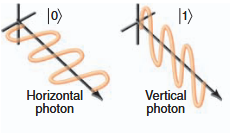
\includegraphics[width=0.5\linewidth]{Photonen_Polarisierung.png}
    \caption{Enter Caption}
    \label{fig:enter-label}
\end{figure}
\cite{obrien_optical_2007}

2. Time-Bin-Encoding 

Photons are chargeless particles, and do not interact very strongly with each other, or even with most matter. They can be guided along long distances with low loss in optical fibers, delayed efficiently using phase shifters, and combined easily using beamsplitters. Photons exhibit signature quantum phenomena, such as the interference produced in two-slit ex- periments. Furthermore, in principle, photons can be made to interact with each other, using nonlinear optical media which mediate interactions 

\textbf{In elektromagnetischem Resonator ist Energie nicht kontinuierlich sondern in units -> “Photonen” -> kleinste Einheiten von Licht / elektromagnetischer Strahlung. }

\textbf{Energiemenge eines Photons hängt von Frequenz der Schwingung ab ℏω (}das reduzierte Plancksche Wirkungsquantum, eine fundamentale Naturkonstant) 

-> in dem Resonator kann es null oder genau ein Photon geben (wie beim Qubit -> Superposition) 

 \cite{nielsen_quantum_2010}
 
\subsection{Spin-Qubits}
\subsection{Neutralatom-Qubits }



Zitat \cite{alhazmi_live_2024}

\cite{bergou_quantum_2021}

\printbibliography
